%---------------------------------------------------------------------------------------------------
%		multi-tenancy.tex
%
%	This is the main file of the chapter that talk about multi-tenancy.
%
%	Author: Andrea Meneghinello
% Version: 0.1
%	Table of changes:
%		12/03/2016 -> document definition
%---------------------------------------------------------------------------------------------------
\section{Multi-tenancy}
\label{sec:elasticity-multiTenancy}
\keyword{Multi-tenancy} refers to a software's architecture principle (or hardware) on which a single instance
of an application is executed inside one (or more) server(s), offering its service to many clients (tenants)
at the same time. The concept must not be confused with the one of multi-instance architecture. The last one
occurs when multiple separated instances (or hardware systems) are made available to different
organizations. Instead, in a multi-tenant architecture the applications are designed to partition 
its data and configurations in a vertical way; every tenant will operate with one of these vertically separated
parts. Figure \ref{img:elasticity-multiTenancy-difference} shows the difference stacks formed by the two
different models.

\begin{figure}
	\centering{}
	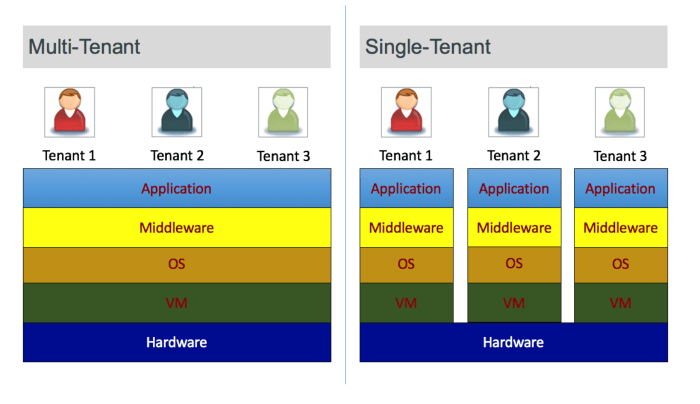
\includegraphics[width=0.65\textwidth]{chapters/elasticity/images/multi-tenancy.png}
	\caption[Multi-teanancy and multi-instance architecture]{The figure shows the difference from a multi-tenant
		architecture and multi-instance one \cite{multiTenancyAnymore}.}
	\label{img:elasticity-multiTenancy-difference}
\end{figure}

Multi-tenancy is a logical consequence of the virtualization technology, on which we can apply a multi-tenant
approach on infrastructure resources. Actually we assist to the creation of logically separated virtual environments
which operate on the same physical components. 

Although the concept itself indicates that there are shared resources (hardware or software), what really
makes the difference is at \keyword{which level resources become multi-tenant}. For example \ac{aws} are
multi-tenant at hardware level because users can be in a state on which they share the same physical
infrastructure. Instead Force.com\footnote{Force.com is a \ac{paas} that allows users to create
multi-tenant add-on applications that will be integrated into the main salesforce.com application.} is rather on
the database level of multi-tenancy because their users share data in the same database's tables. While
Amazon relies on a hypervisor to provide isolation between different tenants (to avoid conflict),
Saleforce.com is based on a query re-writer to achieve the same property.

Multi-tenant software is desirable for software-houses because they can satisfy the needs of different
companies that share a common scenario with one deployed instance and save money due to a reduction
of the number of necessary deployed instances. 

Software-houses do not know a priori the exact number of tenant that will use their applications or services,
hence they require that the \ac{paas} vendor provides them \keyword{good elasticity mechanisms} to be used
with \keyword{elastic software architectures}.

\subsection{Requirements}
\label{sec:elasticity-multiTenancy-requirements}
A good multi-tenant service, deployed by a software-house for many customers, must adhere to the following
requirements:

\begin{itemize}
	\item{\keyword{availability}: the entire service must be redundant in order to ``survive'' to a possible
		malfunctioning of the underlying infrastructure, software errors or both;}
	\item{\keyword{secure isolation}: every tenant must have access only to its data and must not interfere
		with concurrent activities of other tenants; hence the provider must assure, to every customer, that this
		situation cannot happen\footnote{This property can be proved through unit-testing activities that have the
		aim to discover such security lack.};}
	\item{\keyword{guarantee of service}: activities of different tenants must be isolated form each other and it
		is necessary guaranteeing optimal performance both in normal condition, and when some errors occur or in
		presence of workload changes;}
	\item{\keyword{management}: it is essential that software-houses are able to monitor and execute the
		provisioning of all necessary resources in a rapid way in order to maintain the promised service levels
		described in the \ac{sla}.}
\end{itemize}

\subsection{Limits}
\label{sec:elasticity-multiTenancy-limits}
Thanks to a multi-tenant architecture services like Facebook were been able to increase their user-base
in little time. From a developer point of view, a multi-tenant architecture is complicated and can present
some risks:

\begin{itemize}
	\item{\keyword{inflexibility}: if we are deploying a service with sensitive data it is important to
		observe privacy laws; they vary a lot from state to state. In many cases cloud-applications are
		executed in different data-centre to avoid a decline of the offered service, or to prevent a
		possible absence of the offered service. Privacy problems can lead developers in avoiding this paradigm;}
	\item{\keyword{bare security}: if the software is not built and properly tested, it may happen that a
		company may be able to access to data or configurations of other companies; Companies will not migrate to
		our solution if we are not be able to assure that their data are safely safeguarded;}
	\item{\keyword{offered power}: the different companies that benefit of the service may affirm that
		the service is not able to support their workload. \ac{paas} provider, as we just argued, must offer
		good elasticity mechanisms that must be well exploited by the software architecture;}
	\item{\keyword{paradox of having to faces with higher costs}: in many cases the expenditure of re-building
		an entire service or moving data in this new platforms may be not negligible both for software-houses and
		companies.}
\end{itemize}